\chapter{Implementation}
\label{chp:implementation} 

Implementation procedure for mobile robot:

\begin{itemize}

	\item Decide on ROS message interface.
	\item Write interfaces for the motor drivers.
	\item Create a description of the physical structure and properties of the robot in \ac{URDF}. 
	\item Extend the model to enable simulation in Gazebo.
	\item Publish coordinate transform data via \textit{tf} and visualize it in rviz.
	\item Add sensors, with driver and simulation support.
	\item Apply algorithms for navigation and other functionality. 

\end{itemize}

\section{Modelling}

\subsection{Physical Dimensions}

The inertia tensor:

\begin{equation}
    	I = \begin{bmatrix}
    	I_{xx} & I_{xy} & I_{xz} \\[0.3em]
    	I_{yx} & I_{yy} & I_{yz} \\[0.3em]
    	I_{zx} & I_{zy} & I_{zz}
    	\end{bmatrix}
\end{equation}

Inertia tensor for a solid, uniform cylinder where the radius $r$ is measured in parallel to the $x - y$ plane, and $h$ is parallel to the $z$ axis:
\begin{equation}
I_{cylinder} = \frac{1}{12}m \begin{bmatrix}
	(3 r^2 + h^2) & 0 & 0 \\[0.3em]
	0 & (3 r^2 + h^2) & 0 \\[0.3em]
	0 & 0 & r^2
	\end{bmatrix}
\end{equation}

Inertia tensor for a solid, uniform cuboid. The subscript of $l$ indicates which axis $l$ is measured along:
\begin{equation}
I_{cuboid} = \frac{1}{12}m \begin{bmatrix}
	(l_y^2 + l_z^2) & 0 & 0 \\[0.3em]
	0 & (l_x^2 + l_z^2) & 0 \\[0.3em]
	0 & 0 & (l_x^2 + l_y^2)
\end{bmatrix}
\end{equation}

\subsection{Coordinate Frames}

\section{Simulations}

\section{ROS Nodes for Motion Control}

\begin{figure}[p]
	\centering
	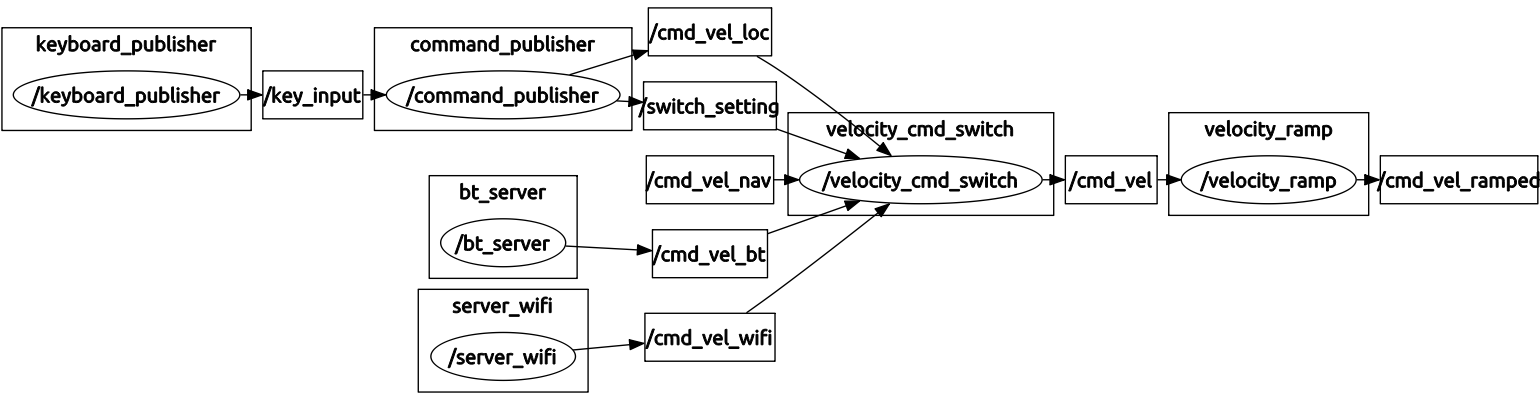
\includegraphics[width=1\textwidth]{move_base_nodes}
	\caption{Nodes and topics for motion control. }
	\label{fig:move_base_nodes}
\end{figure}

\section{Operator Control Station (OCS)}

The \ac{OCS} allows an operator to control and monitor the robot through a graphical user interface. \texttt{MainWindow}

\subsection{Graphical User Interface}

A Qt-based \ac{GUI}...

\section{The Handheld Remote Control - "Robot Leash"}

http://developer.samsung.com/technical-doc/view.do?v=T000000117
